\input{style/settings}
\input{style/short_commands}
\pagestyle{fancy}
\fancyhf{}
\fancyhead[R]{página\;\thepage/\pageref{LastPage}}
\fancyhead[L]{Osvaldo Uriel Calderón Dorantes}
\fancyfoot[L]{Imagenología Biomédica}
\fancyfoot[R]{Facultad de Ciencias, UNAM 
\includegraphics[scale=0.13]{style/Sheikah.pdf}}
\fancypagestyle{plain}{
  \fancyfoot[C]{}
}
\makeatletter
\def\@seccntformat#1{%
  \expandafter\ifx\csname c@#1\endcsname\c@section\else
  \csname the#1\endcsname\quad
  \fi}
\makeatother
%%%%%%%%%%%%%%%%%%%%%%%%%%%%%%%%%%%%%%%%%%%%%%%%%%%%%%%
%%%%%%%%%%%%%%%%%%%%%%%%%%%%%%%%%%%%%%%%%%%%%%%%%%%%%%%%%%%
\begin{document}
\begin{flushleft}
Osvaldo Uriel Calderón Dorantes, \hfill Imagenología Biomédica\\
316005171 \hfill osvaldo13576@ciencias.unam  \\
Facultad de Ciencias\\
\underline{Universidad Nacional Autónoma de México}
\end{flushleft}

\begin{flushright}\vspace{-5mm}

\includegraphics[height=1.5cm]{style/logo.pdf}
\end{flushright}
 
\begin{center}\vspace{-1cm}
\textbf{ \large \customfont{Evaluación\\
Módulo Ultrasonido}}\\
\today
\end{center}
%\medskip\hrule\medskip
%%%%%%%%%%%%%%%%%%%%%%%%%%%%%%%%%%%%%%%%%%%%%%%%
%{\small \textbf{Nota: A las unidades las pondré dentro de corchetes \ec{[\tx{unidad}]} para no confundir entre variables y realizar el análisis dimensional fácilmente.}}
\medskip\hrule\bigskip

\newlength{\strutheight}
\settoheight{\strutheight}{\strut}
\begin{enumerate}
  \item Describir detalladamente efecto piezoeléctrico, cómo éste se aplica en la generación de energía ultrasónica para diagnóstico médico y cuáles son las características de las cerámicas o cristales piezoeléctricos que determinan la frecuencia natural de oscilación.
  
  El efecto piezoeléctrico en cristales se refiere a la aparición de carga eléctrica en sus superficies cuando son comprimidos o estirados, estos cristales son llamados piezoeléctricos \citep{WHO}.
    
    \begin{adjustbox}{valign=T,raise=\strutheight,minipage={\linewidth}}
      \begin{wrapfigure}{r}{0.6\textwidth}
        \centering
        \captionsetup{margin=5pt}
        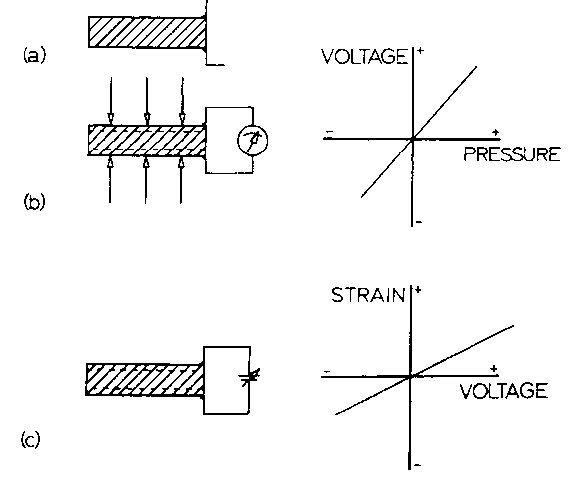
\includegraphics[width=0.4\textwidth]{./figuras/p1_0.pdf}
        \caption{Diagrama de generación de voltaje por deformación mecánica. La figura se recuperó de \citet{matthew}.}
        \label{p1:0}
      \end{wrapfigure}
    \strut{}  
    
    En la figura \hyperref[p1:0]{\ref{p1:0}.(a)} se puede observar la representación de un cristal piezoeléctrico en donde se considera que éste es un disco plano el cual tiene electrodos en ambas caras paralelas. Este material produce un voltaje con cierta polaridad cuando se ejerce una presión, de manera que cuando cambia de sentido la presión, el voltaje invierte su polaridad y de acuerdo a la figura, la presión es directamente proporcional al voltaje de tal manera que cuando se indice una presión alternante, el voltaje cambiará su polaridad de manera sinusoidal, lo cual se presenta en el gráfico de la figura \hyperref[p1:0]{\ref{p1:0}.(b)}. Otro caso que puede ocurrir es el efecto piezoeléctrico inverso donde el cristal se conecte a una fuente externa de voltaje el cual le produce un cambio de tensión, teniendo que el voltaje es directamente proporcional a la tensión generada, este comportamiento se presenta en el gráfico de la figura \hyperref[p1:0]{\ref{p1:0}.(c)} \citep{matthew}. 



    \end{adjustbox}

    De lo anterior se resume que en el segundo caso puede ser empleado para la generación de ondas mecánicas de ultrasonido y en el primer caso para su detección, entonces se busca que la señal con una frecuencia de oscilación dada genere otra a la misma frecuencia a través del transductor ofreciendo la respuesta máxima, la cual es llamada frecuencia natural o fundamental \ec{f_0} \citep{matthew}.
    
    




    \begin{adjustbox}{valign=T,raise=\strutheight,minipage={\linewidth}}
      \begin{wrapfigure}{l}{0.6\textwidth}
        \centering
        \captionsetup{margin=5pt}
        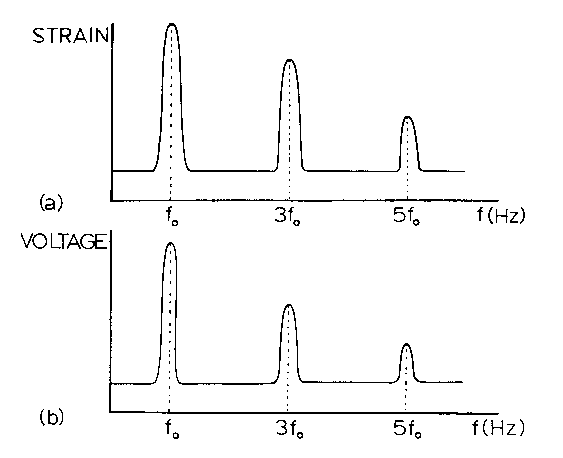
\includegraphics[width=0.4\textwidth]{./figuras/p1_1.pdf}
        \caption{Comportamiento de resonancia de un disco piezoeléctrico. La figura se recuperó de \citet{matthew}.}
        \label{p1:1}
      \end{wrapfigure}
    \strut{}  
    
    La geometría de los transductores más comunes son las circulares y la semicirculares, también hay de geometría rectangular, y un parámetro importante es el grosor del disco ya que determina la frecuencia de máxima sensibilidad de este. Entonces si tenemos un grosor constante con un voltaje de entrada alternante de amplitud constante pero frecuencia variable, se observa el comportamiento en el gráfico de la figura \hyperref[p1:1]{\ref{p1:1}.(a)} el cual nos muestra cómo se comporta la amplitud de deformación, de donde se tiene la máxima amplitud en los armónicos impares, dado en la ecuación \ref{e:p1:0}.
    \eq{e:p1:0}{f_0=\dfrac{c}{2d}}

  \end{adjustbox}

\pagebreak

También la ecuación \ref{e:p1:0} podemos obtener el grosor en función de la frecuencia o de la longitud de onda, obteniendo la ecuación \ref{e:p1:1}.
\begin{equation}
  \begin{split}
    d&=\dfrac{c}{f_0}\\
  &=\dfrac{\lambda_0}{2}
  \end{split}
  \label{e:p1:1}
\end{equation}
Donde \ec{f_0} es la frecuencia natural, \ec{c} es la velocidad de propagación y \ec{\lambda_0} es la longitud de onda natural, de esta expresión se obtiene la resonancia de media longitud de onda para el cristal. Por último cuando el piezoeléctrico se usa en el modo recíproco cuando detecta el ultrasonido, producirá un voltaje con picos en las mismas frecuencias como se muestra en la figura \hyperref[p1:1]{\ref{p1:1}.(b)} \citep{matthew,IM}

  Otra característica a considerar es la densidad, ya que la ecuación de onda que modela la perturbación transversal en una cuerda involucra la velocidad de esta perturbación como se muestra en la ecuación \ref{e:p1:2} donde \ec{\rho} es la densidad del material y \ec{T} es la tensión, de esta forma se obtiene los armónicos descritos en la ecuación ecuación \ref{e:p1:3} que nos dice que la frecuencia más lentas es para densidades grandes y que la frecuencia puede ser controlada alternando la tensión ya que la frecuencia aumenta conforme aumente la tensión \citep{haim}.
\eq{e:p1:2}{\dfrac{\partial^2 y}{\partial x^2}=\dfrac{1}{c^2}\dfrac{\partial^2 y}{\partial t^2},\quad c=\sqrt{\dfrac{T}{\rho}}}
\eq{e:p1:3}{f_n=\dfrac{n}{2d}\sqrt{\dfrac{T}{\rho}}}


  \item Describir detalladamente la variación de presión acústica en el campo cercano y lejano.
  
  
  
  \begin{adjustbox}{valign=T,raise=\strutheight,minipage={\linewidth}}
    \begin{wrapfigure}{l}{0.6\textwidth}
      \centering
      \captionsetup{margin=5pt}
      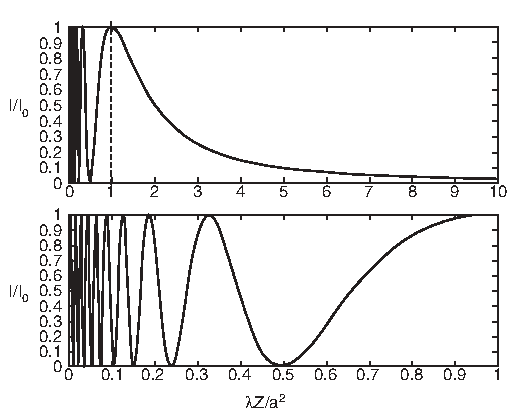
\includegraphics[width=0.5\textwidth]{./figuras/p2_0.pdf}
      \caption{Variación en el campo cercano y lejano, donde la intensidad \ec{I} se ha normalizado con respecto a \ec{I_0} y la distancia \ec{z} con respecto a \ec{\lambda z/a^2}. La figura se recuperó de \citet{haim}.}
      \label{p2:0}
    \end{wrapfigure}
  \strut{}  
  
 Dado que la intensidad de una onda acústica está relacionada con la presión máxima \ec{P_{\tx{máx}}}, ecuación \ref{e:p2:0}, con \ec{\rho} la densidad del material y \ec{c} la velocidad del sonido \citep{russ}
 \eq{e:p2:0}{I=\dfrac{{P_{\tx{máx}}}^2}{2\rho c}}
Sin embargo, \citet{haim} proporcionan una relación, ec. \ref{e:p2:1}, donde \ec{I} e \ec{I_0} son las intensidades en el punto \ec{z} y en la fuente, respectivamente, \ec{\lambda} es la longitud de onda correspondiente en el medio y \ec{a} es el radio del transductor el cual tiene geometría de disco:
\eq{e:p2:1}{\dfrac{I}{I_0}=\sin^2\cor{\dfrac{\pi}{\lambda}\p{\p{a^2+z^2}^{1/2}-z}},}
además, dado que es una función periódica, sus valores máximos y mínimos alternan, los puntos que dan un máximo se describen en la ecuación \ref{e:p2:2}, mientras que los mínimos aparecen en los puntos de la ecuación \ref{e:p2:3}.
\eq{e:p2:2}{z_{\tx{máx}}=\dfrac{4a^2-\lambda^2(2m+1)^2}{4\lambda(2m+1)},\quad m=0,\;1,\;2,...}
\eq{e:p2:3}{z_{\tx{mín}}=\dfrac{a^2-\lambda^2n^2}{2n\lambda},\quad n=1,\;2,\;3,...}

\end{adjustbox}

Ya descrito lo anterior, de acuerdo con la figura \ref{p2:0} se puede observar que antes del punto \ec{\lambda Z/a^2=1} la intensidad cambia drásticamente y por ello no es conveniente realizar mediciones e imágenes, pues, además, es difícil determinar si las amplitudes de los ecos provienen de discontinuidades de las propiedades del medio o de las variaciones del campo acústico; esta región se llama campo cercano. Después del campo cercano, el campo acústico se vuelve más predecible ya que comienza a decaer monótonamente y su uso para la medición entones es más conveniente, esta región se llama campo lejano.

  

\pagebreak


  \item ¿Hay alguna relación de la frecuencia natural de oscilación, respecto a la dispersión del campo de visión, a la zona de transición entre los campos cercano y lejanos, al decaimiento de la energía con respecto a la distancia de penetración y a las resoluciones lateral y axial del haz?
  
 







  \item ¿Cuáles son las diferencias, referente a la dispersión acústica, entre un arreglo lineal, arreglo en dos dimensiones, arreglo curvilíneo y arreglo en fase? Describir detalladamente cada uno de ellos.

  
  \begin{figure}[!ht]
    \centering
    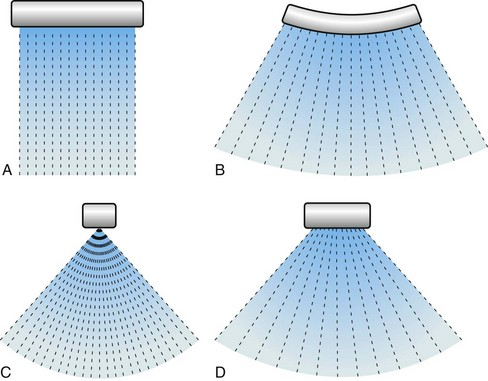
\includegraphics[width=0.4\textwidth]{./figuras/transductores_radiokey.jpg}
    \caption{Arreglo lineal (A), arreglo curvilíneo (B)  arreglo en fase (C) y arreglo en dos dimensiones (D). La figura re recuperó de la web de \citet{radiokey1}.}
    \label{transductores_radiokey}
  \end{figure}

La dispersión acústica ocurre en objetos que tienen el tamaño de la longitud de onda o más pequeños, también de forma irregular dependen menos del ángulo, aunque son menos intensos \citep{halliwell}. La geometría de los haces darán un efecto de dispersión acústica distinto, con el arreglo lineal tendremos una mayor dispersión en las zonas superficiales y, en los curvilíneos y arreglos en fase se dará la dispersión en las zonas más profundas ya que es ahí en ambos casos se tiene mejor resolución espacial.






  \item Qué importancia tienen los lóbulos laterales en la generación de la imagen ultrasónica. Describir detalladamente los efectos.
  
  \begin{adjustbox}{valign=T,raise=\strutheight,minipage={\linewidth}}
    \begin{wrapfigure}{r}{0.6\textwidth}
      \centering
      \captionsetup{margin=5pt}
      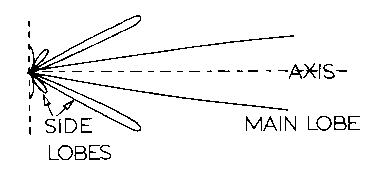
\includegraphics[width=0.5\textwidth]{./figuras/p3_0.pdf}
      \caption{Generación de lóbulos. La figura se recuperó de \citet{matthew}.}
      \label{p5:0}
    \end{wrapfigure}
  \strut{}  
  
A pesar que el haz de ultrasonido sea enfocado, hay una fuga de energía dando lugar el surgimiento de los lóbulos laterales (side-lobes) los cuales provocan una degradación en la imagen \citep{kun}. Además, en el campo lejano se tienen un par de limitantes, una de estas es que el lóbulo principal (main lobe) es la divergencia como se observa en la figura \ref{p5:0} y la otra es el surgimiento de los lóbulos laterales que, por conservación de energía, que toman parte de la energía y no van dirigidos a lo largo del eje del lóbulo principal \citep{matthew}.



\end{adjustbox}

Los lóbulos laterales producen artefactos, el objeto se representa de manera incorrecta en la pantalla como resultado de los ecos producidos por estos lóbulos que acompañan al lóbulo principal, la cual se puede ver como una línea curva en una estructura anecoica y se pueden confundir con ecos internos en órganos quísticos. Este artefacto puede ser eliminado fácilmente si se inclina ligeramente el transductor o cambiando el plano de exploración \citep{thieme}.


  


  \item ¿Consideras importante hacer un pre-procesamiento de las señales adquiridas y por qué?
  
Sí. El pre-procesamiento es importante pues permite una mejora en la calidad y la resolución de la señal al momento de recibir los ecos \citep{thieme}. \citet{russ} explican que hay distintos factores por los cuales se requiere un proceso de pre-procesamiento los cuales se resumen en el desajuste de impedancia acústica en la interfaz en donde se generó la señal, la atenuación de los tejidos intermedios y la amplitud del pulso de ultrasonido, los cuales hacen que varíe la amplitud del eco registrado. La atenuación de esta amplitud es compensada por un circuito de compensación de ganancia de tiempo (TGC), o veces llamado compensación de ganancia de profundidad (DGC) o circuito de ganancia variable en el tiempo (TVG), el cual usa la relación entre la profundidad y el tiempo de llegada del eco al transductor, entonces los ecos que regresan en tiempos más largos, y por ende desde una mayor profundidad, reciben una mayor ganancia compensando la atenuación por el tejido blando.

  \item Cuáles son los parámetros importantes para la generación de la imagen de Modo B? Describir cada uno de ellos.
  
  \citet{godau_berg_2013} explican que los parámetros técnicos que se deben considerar para la generación de la imagen, al menos para estudios de ultrasonografía transcraneal, son \citep{matthew}: 
  
  
    
\begin{itemize}
  \item Un equipo de gama alta con transductores de frecuencia natural de \ec{1.5} a \ec{3.5\un{Hz}} de arreglo en fase.
  \item Se debe tener una resolución espacial axial (la capacidad para distinguir los ecos de dos superficies reflectantes cercanas a lo largo del eje del haz) de aproximadamente \ec{0.7\un{mm}}  y una lateral (la capacidad de distinguir en la imagen dos reflectores vecinos colocados uno cerca del otro) de aproximadamente \ec{1.05\un{mm}}.
  \item Profundidad de penetración de \ec{14} a \ec{16\un{cm}} para abarcar mayor superficie de estudio.
  \item  Rango dinámico de \ec{45} a \ec{60\un{dB}}, el cual se refiere al rango de ganancia inicial en decibeles hasta que la señal se sature.
  \item Tasa de imagen bajo, ya que los cambios fisiológicos para este tipo de estudio son muy lentos.
\end{itemize}

  \item Para generar la imagen en 2D se requiere procesar digitalmente las señales adquiridas, si es así ¿cuales?
  




  \item Describir detalladamente el efecto Doppler y la información que nos ofrece el ultrasonido Doppler. Cuáles son los parámetros importantes para el estudio médico de Doppler a color y la importancia de ello.
  

\begin{adjustbox}{valign=T,raise=\strutheight,minipage={\linewidth}}
  \begin{wrapfigure}{r}{0.6\textwidth}
    \centering
    \captionsetup{margin=5pt}
    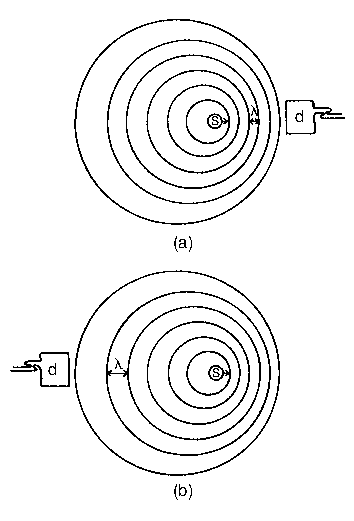
\includegraphics[width=0.3\textwidth]{./figuras/p9_0.pdf}
    \caption{Efecto Doppler. La figura se recuperó de \citet{russ}.}
    \label{p9:0}
  \end{wrapfigure}
\strut{}  

El efecto Doppler es la ocurrencia de un cambio de frecuencia observada de una onda de sonido o ultrasonido cuando hay un movimiento entre  la fuente de sonido y el observador. En el caso de la ecografía clínica, tendremos dos desplazamientos Doppler si un reflector en movimiento se encuentra en el haz de un transductor de fuente fija idealmente, por lo que produce un segundo cambio Doppler en frecuencia, igual en magnitud al primer cambio \citep{matthew}. 

Como se observa en la figura \ref{p9:0}  el cambio de frecuencia se da cuando una fuente de ultrasonido se mueve a velocidad \ec{v_s} hacia el detector d, después de un tiempo \ec{t} sigue la producción de un frente de onda cuya distancia entre el frente de onda y la fuente es \ec{(c-v_s)t} con \ec{c} la velocidad del ultrasonido en el medio, de modo que la longitud de onda para este caso se describe por la ecuación \ref{e:p9:0}, con \ec{\nu_0} la frecuencia del ultrasonido desde la fuente, así, la frecuencia cambia a un valor más alto cuando el ultrasonido se desplaza hacia el detector teniendo que el cambio de frecuencia está dada por la ecuación \ref{e:p9:1}. El otro caso es cuando la frecuencia cambia a un valor más bajo cuando la fuente de ultrasonido se aleja del detector, por lo que la ecuación de la frecuencia cambia como se describe en la ecuación \ref{e:p9:2}.
\eq{e:p9:0}{\lambda=\dfrac{c-v_s}{\nu_0}}
\eq{e:p9:1}{\Delta \nu=\nu-\nu_0=\nu_0\p{\dfrac{c}{c-v_s}}-\nu_0=\nu_0\p{\dfrac{v_s}{c-v_s}}}
\eq{e:p9:2}{\Delta \nu=\nu-\nu_0=\nu_0\p{\dfrac{v_s}{c+v_s}}-\nu_0=\nu_0\p{\dfrac{-v_s}{c+v_s}}}
\end{adjustbox}


\pagebreak

  \item Describir detalladamente los siguientes términos en una imagen ultrasónica: (i)  Ecogenicidad, (ii) Hiperecoico, (iii) Isoecoico, (iv) Hipoecoico, (v) Anecoico.
  
\begin{itemize}%http://famus.org.uk/modules/ultrasound-theory-module
  \item \textbf{Ecogenicidad}. Se refiere a la capacidad de generar ecos \citep{famus}.
  \item \textbf{Hiperecoico}. Es un material que es altamente reflectante y es más brillante a diferencia de otras estructuras vecinas.
  \item \textbf{Isoecoico}. Material el cual tiene ecogenicidad similar a las estructuras circundantes.
  \item \textbf{Hipoecoico}. Es menos reflectante y por lo tanto menos brillante que el material circundante.
  \item \textbf{Anecoico}. Material que no produce eco, careciendo de color. En imágenes de US este material se observa de color negro.
\end{itemize}

\end{enumerate}








\begin{multicols}{2}
\small{\bibliographystyle{apalike}
\bibliography{bib}}
\end{multicols}



%\ftikz{1.5}{figuras/fig.tikz}{}{fig:x}

\end{document}